\input{preamble.tex}

% --------------------------------------------------------------------
% --------------------------------------------------------------------
% ---- ENTER YOUR PROJECT DETAILS BELOW

% ---- title of the project
\title{Curriculum Graph: Student-Centric Curriculum Planning with Dependency Analytics}

% ---- names of team members
\author{
    \small Ayush Raj \and
    \small Malhar Patel \and
    \small Sankar Maharajan \and
    \small Applen Tahu
    }

% ---- enter the team number below
\rhead{Curriculum Graph Team}

% --------------------------------------------------------------------
% --------------------------------------------------------------------


% --------------------------------------------------------------------
% --------------------------------------------------------------------
% ---- DO NOT CHANGE THIS BLOCK OF CODE
\begin{document}
\maketitle
% --------------------------------------------------------------------
% --------------------------------------------------------------------



% --------------------------------------------------------------------
% --------------------------------------------------------------------
% ---- WRITE YOUR REPORT BELOW

% Helper macros for optional local screenshots.
% If an image is missing, a placeholder box is shown instead of failing compile.
\newcommand{\safeincludegraphics}[1]{%
    \IfFileExists{#1}{%
        \includegraphics[width=\textwidth]{#1}%
    }{%
        \fbox{\parbox[c][0.48\textwidth][c]{0.95\textwidth}{\centering
            Missing figure:\\
            \path{#1}
        }}%
    }%
}

\newcommand{\safeincludegraphicsalt}[2]{%
    \IfFileExists{#1}{%
        \includegraphics[width=\textwidth]{#1}%
    }{%
        \IfFileExists{#2}{%
            \includegraphics[width=\textwidth]{#2}%
        }{%
            \fbox{\parbox[c][0.48\textwidth][c]{0.95\textwidth}{\centering
                Missing figure:\\
                \path{#1}\\
                (or)\\
                \path{#2}
            }}%
        }%
    }%
}

\section{Introduction}
We developed \textit{Curriculum Graph}, a student-centric dashboard for
major/minor planning that combines prerequisite dependency analytics with an
interactive UI. The system helps students understand course dependencies,
validate program requirements, and plan feasible semesters under offering and
credit constraints.

Curriculum planning is often difficult for students because prerequisite
relationships, semester offerings, and major/minor rules are spread across
multiple documents. A graph-based representation is naturally suited for this
problem: courses are modeled as nodes and prerequisites as directed edges.
Graph traversal, topological logic, and bottleneck analysis then become useful
for practical advising and semester-by-semester planning \citep{networkx_2008}.

The main challenge is not only algorithmic; it is also usability. Even a
correct graph can be hard to use if the interface is cluttered or if required
insights are buried in technical detail. We therefore combine backend graph
analytics with a student-facing dashboard built in Streamlit \citep{streamlit}
and yFiles for interactive graph rendering \citep{yfiles_streamlit}.


\section{Problem Statement and Objectives}
Our goal is to build a reproducible, policy-aware planning system that answers
the following student questions:

\begin{itemize}
    \item What should I take next semester given my completed courses?
    \item Which prerequisites are blocking my progress?
    \item Is my current pathway valid for my major and minor?
    \item Can I still reach the degree target under term constraints?
\end{itemize}

The concrete objectives are:

\begin{itemize}
    \item Build clean dependency graphs with semester and year structure.
    \item Validate major/minor pathways against rule sets.
    \item Generate constrained semester plans (course and credit caps).
    \item Provide an accessible UI with student mode and advanced mode.
    \item Ensure reliability through testing, validation checks, and a clean
    modular code structure.
\end{itemize}

\section{Methods}
\subsection{Data}
The system uses three primary JSON inputs:

\begin{itemize}
    \item Course catalog: course code, name, credits, subject, kind,
    prerequisites, and semester offerings.
    \item Major/minor requirement rules: set-wise constraints and exclusions.
    \item College constraints: number of semesters and minimum degree credits.
\end{itemize}

In the current snapshot, the dataset contains 264 courses, 9 subjects, and 16
major/minor criteria entries \citep{iiser_data}. Data-health checks report no
duplicate course codes, no missing prerequisite links, and no unknown
requirement codes.

\subsection{Implementation Summary}
The final codebase is organized into clear modules:

\begin{itemize}
    \item \texttt{src/app.py}: Streamlit dashboard and interaction logic.
    \item \texttt{src/graph.py}: graph construction, planning, and analytics
    utilities.
    \item \texttt{src/validate\_major\_minor.py}: rule validation and
    requirement checks.
\end{itemize}

This structure enabled a maintainable workflow where UI improvements and
algorithmic improvements could be developed independently and then integrated.

\subsection{Data Quality and Rule Validation}
Before graph construction and planning, we run a quality report over both the
course catalog and the major/minor rule JSON. These checks are intended to
catch data issues that would otherwise mislead students.

The quality report flags:
\begin{itemize}
    \item duplicate course codes and duplicate program-rule entries,
    \item missing prerequisite links (a prerequisite code not present in the catalog),
    \item self-prerequisites (a course listing itself as a prerequisite),
    \item missing semester-offering tags,
    \item unknown requirement codes inside Set A--E rule lists.
\end{itemize}

The major/minor rules are encoded as a set-based schema:
\begin{itemize}
    \item \textbf{Set D}: compulsory courses that must be included,
    \item \textbf{Set A}: elective pool with a minimum selection requirement,
    \item \textbf{Set B}: elective pool with a maximum allowed cap,
    \item \textbf{Set C}: supplementary pool that can contribute to totals,
    \item \textbf{Set E}: courses that are excluded (not counted) from totals.
\end{itemize}

In addition to set-wise constraints, the validator checks overall minimum
course-count and credit requirements. The dashboard reports both the student
input totals and the counted totals after applying Set E exclusions.

Requirement validation is performed set-wise (Sets A/B/C/D/E) and overall
(minimum courses and minimum credits). Additionally, we support a
prerequisite-completeness check that can be configured as \textit{strict}
(treated as errors), \textit{advisory} (treated as warnings), or \textit{off}
(ignored). This prevents students from accidentally selecting advanced courses
without ensuring all prerequisites are included in their plan.

\subsection{Graph Modeling and Planning}
We build a directed graph $G=(V,E)$ where $V$ is the selected course set and
$E$ contains edges $(u,v)$ whenever course $u$ is a prerequisite of course $v$.
The planning engine uses semester offerings and prerequisite satisfaction to
select feasible courses term-by-term.

At a high level, the semester planner greedily selects available courses while
respecting per-term caps and prioritizing compulsory requirements. The process
is described in Algorithm~\ref{alg:planner}.

For each course $c$, feasibility in semester $s$ is defined by two conditions:
offering availability and prerequisite satisfaction,
\begin{align}
    c \in \mathcal{O}(s), \label{eq:offering}\\
    \mathrm{pred}(c) \subseteq \mathcal{C}_{\mathrm{done}}, \label{eq:prereq}
\end{align}
where $\mathcal{O}(s)$ is the set of courses offered in semester $s$, and
$\mathcal{C}_{\mathrm{done}}$ is the completed course set.

\subsubsection{Graph Integrity Checks (Cycle / Loop Detection)}
Since prerequisite graphs must be acyclic to support strict scheduling, we
explicitly detect directed cycles (loops) in the prerequisite graph. If any
cycle is present, the dashboard highlights the cycle and the constrained
planner exits early with a clear reason. When the graph is a DAG, we compute a
topological order to provide a prerequisite-respecting sequence.

We also compute reachability from start-feasible root nodes (courses with no
incoming prerequisites and at least one offering at/after the chosen start
semester). Unreachable nodes indicate either offering constraints or a
prerequisite chain that cannot be satisfied under the selected horizon.

Finally, we compute bottleneck indicators (downstream reach and betweenness
centrality) to identify high-impact courses that unlock many others.

\subsection{Dashboard Design}
The dashboard has two usage modes:

\begin{itemize}
    \item \textbf{Student mode}: fewer tabs, cleaner defaults, readable labels,
    and within-year arrow emphasis.
    \item \textbf{Advanced mode}: full algorithm diagnostics, rule explorer,
    validation internals, and quality views.
\end{itemize}

To reduce cognitive overload, graph legends are explicit, transition summaries
are collapsible, and major/minor options are policy-filtered to approved
offerings in the current deployment profile.

The UI uses progressive disclosure: essential views are visible by default,
while heavier diagnostics are placed behind toggles/expanders. A key
readability feature is the \textit{Graph Clarity Controls}, which let users
choose (i) a visual density profile, (ii) label detail level, (iii) whether to
show all prerequisite arrows or only within-year arrows, and (iv) layout style
(hierarchic/orthogonal/organic/tree). This makes the same underlying graph
usable for both quick planning and deeper debugging.

Interactive selection is central to the design: clicking nodes reveals course
metadata (credits, offerings, subject/kind) and requirement-role labels (e.g.,
compulsory vs elective pool). This reduces the need to cross-reference external
documents while planning.

\subsection{Testing and Robustness}
Reliability was treated as a first-class requirement because students interact
with the system through an embedded graph renderer. The dashboard wraps graph
rendering calls in a safe execution path that surfaces errors without breaking
the entire page. On the analytics side, cycle detection prevents the planner
from producing invalid schedules, and quality reports help identify catalog
issues (missing prerequisites, duplicates, missing offerings) early. We also
use lightweight smoke tests (syntax checks and headless app startup) to ensure
the app remains runnable across machines.

\section{Results}
\subsection{Quantitative Summary}
Table~\ref{tab:summary} reports key metrics from the latest run.

\begin{table}[tbp]
    \centering
    \caption{Dataset and system summary statistics.}
    \label{tab:summary}
    \begin{tabular}{|l|c|}
        \hline
        Metric & Value \\
        \hline
        Total courses & 264 \\
        Program entries (major/minor) & 16 \\
        Subjects covered & 9 \\
        Prerequisite edges & 94 \\
        Average credits per course & 3.42 \\
        Missing prerequisite links & 0 \\
        Unknown requirement-code hits & 0 \\
        \hline
    \end{tabular}
\end{table}

\subsection{Delivered System Features}
The following deliverables were completed and validated in the current version:

\begin{itemize}
    \item Student mode and advanced mode toggles for clean navigation.
    \item Policy-filtered major/minor options for institutional constraints.
    \item Year-semester structured prerequisite graphs with readable labels.
    \item Semester transition summaries for better planning visibility.
    \item Graph integrity checks: cycle (loop) detection, DAG/topological order
    diagnostics, and reachability summaries.
    \item Constrained term-by-term planner with blocked-course diagnostics.
    \item Bottleneck analytics (downstream reach and betweenness) to identify
    high-impact prerequisite courses.
    \item Major-minor combination simulator for comparative pathway analysis.
    \item Data quality checks and pathway validation reports.
\end{itemize}

\begin{figure}[tbp]
    \centering
    \IfFileExists{./figs/major_minor_overview.png}{%
        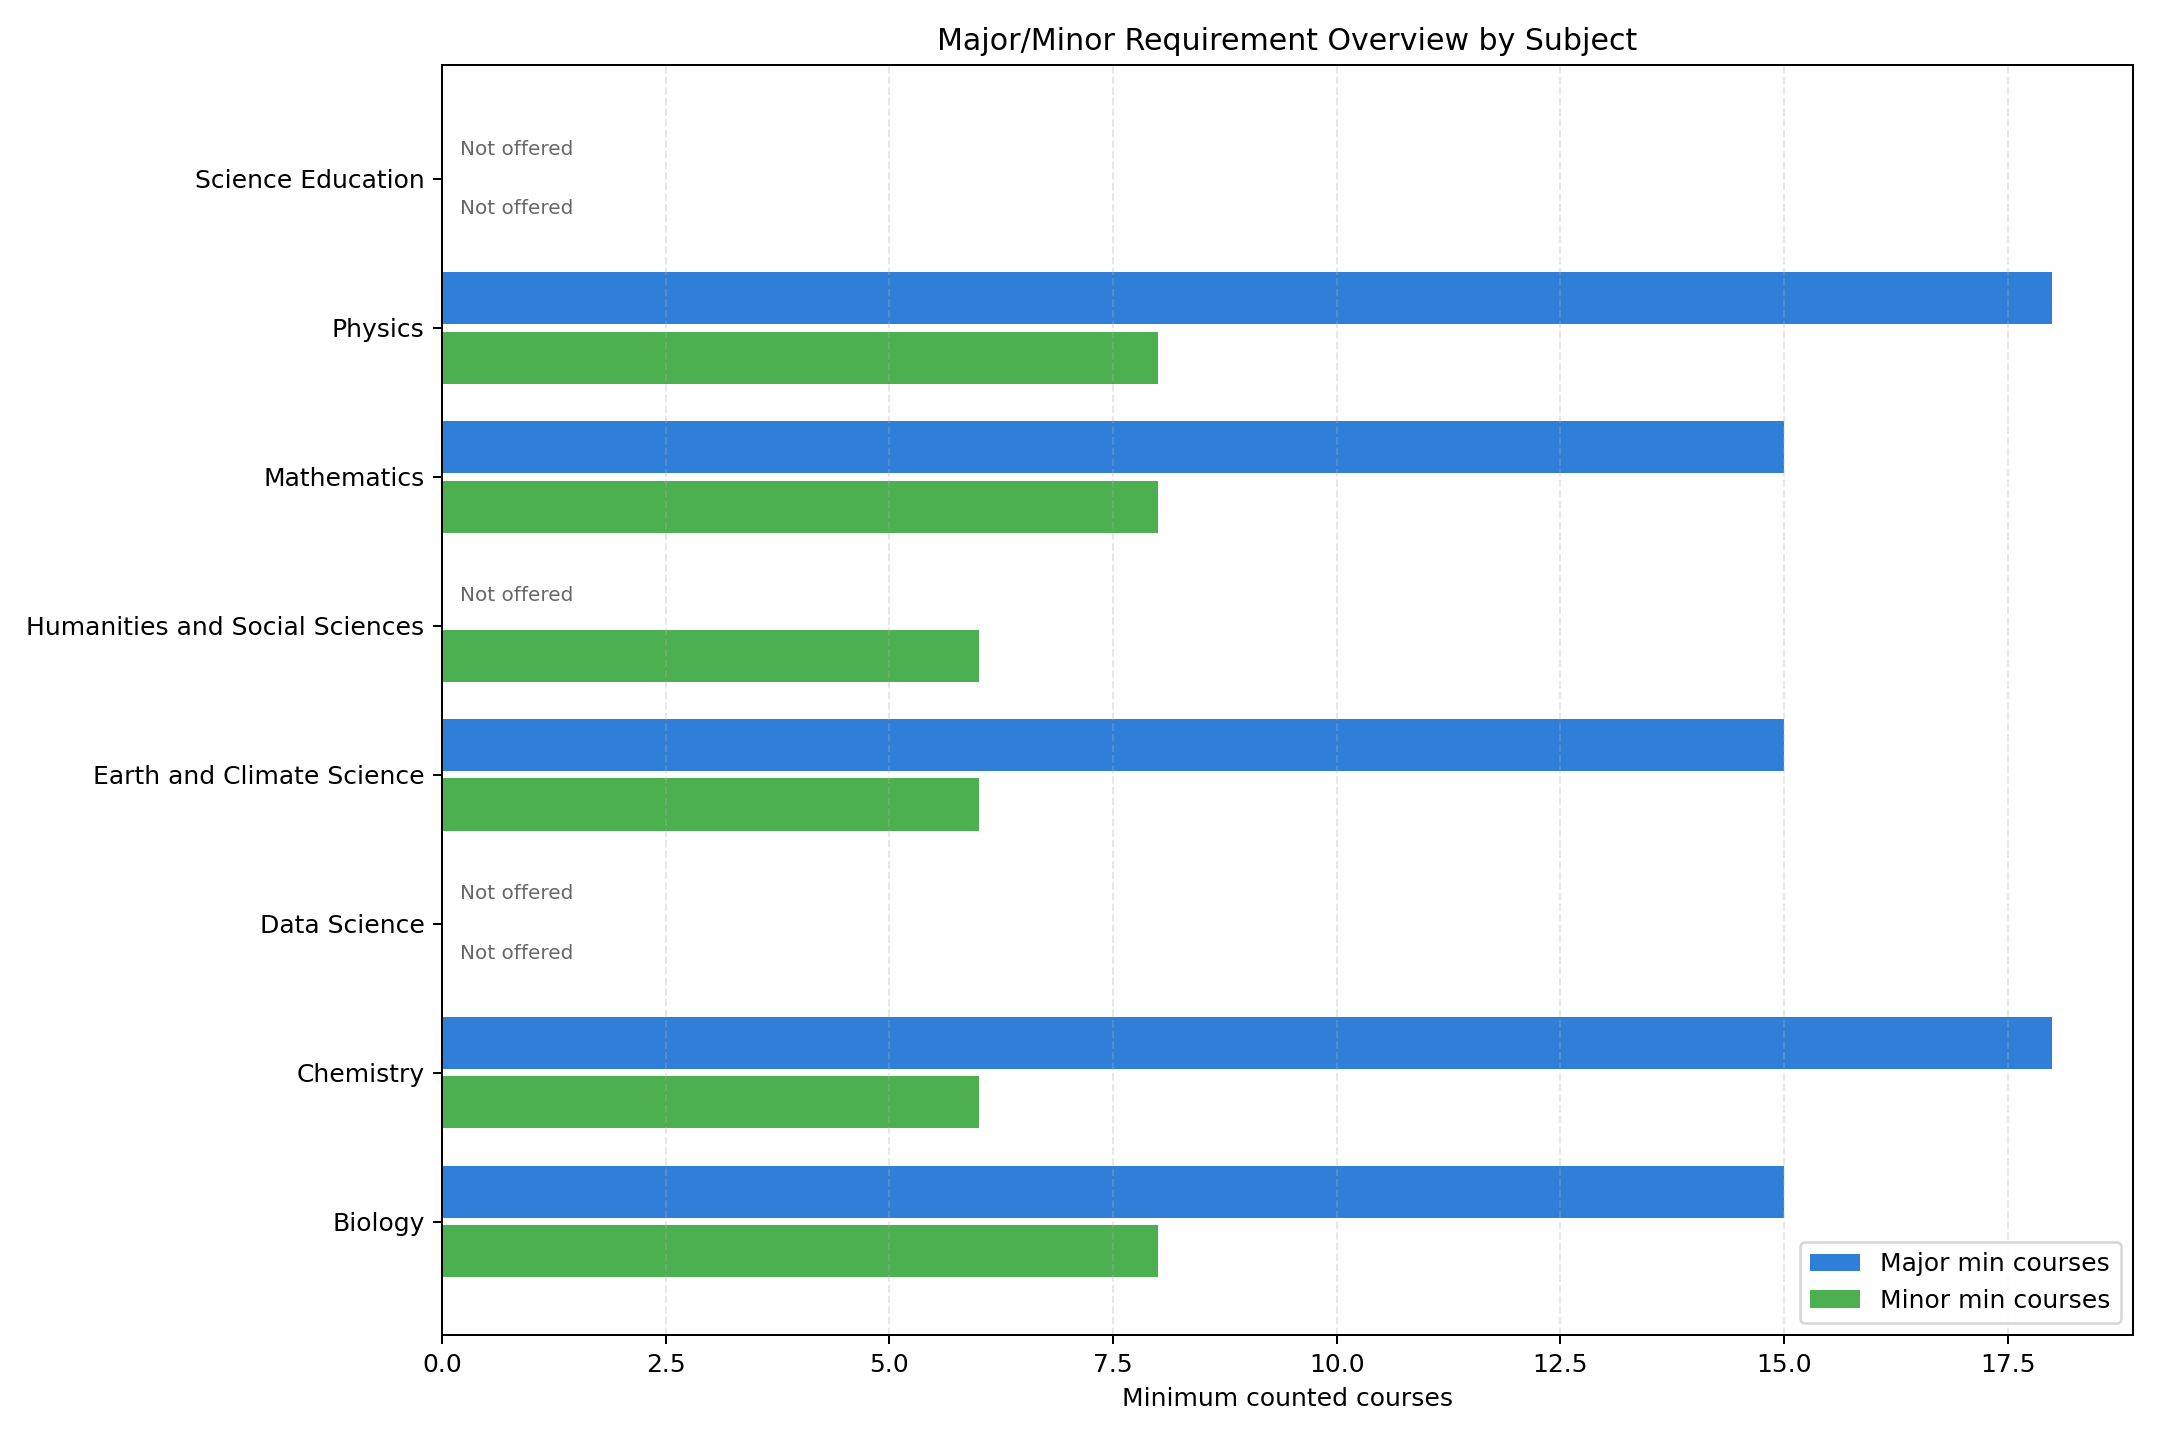
\includegraphics[width=0.92\textwidth]{./figs/major_minor_overview.png}%
    }{%
        \fbox{\parbox[c][0.35\textwidth][c]{0.85\textwidth}{\centering
            Missing figure:\\
            \path{./figs/major_minor_overview.png}
        }}%
    }
    \caption{Overview of major-minor requirement structure used in the planning system.}
    \label{fig:majmin-overview}
\end{figure}

\subsection{Visual Analytics and Plots}
Figure~\ref{fig:sem-year} shows the course distribution by semester and year,
while Fig.~\ref{fig:subject-patterns} shows subject-level and prerequisite
structure patterns.

\begin{figure}[tbp]
    \centering
    \begin{minipage}{0.48\textwidth}
        \centering
        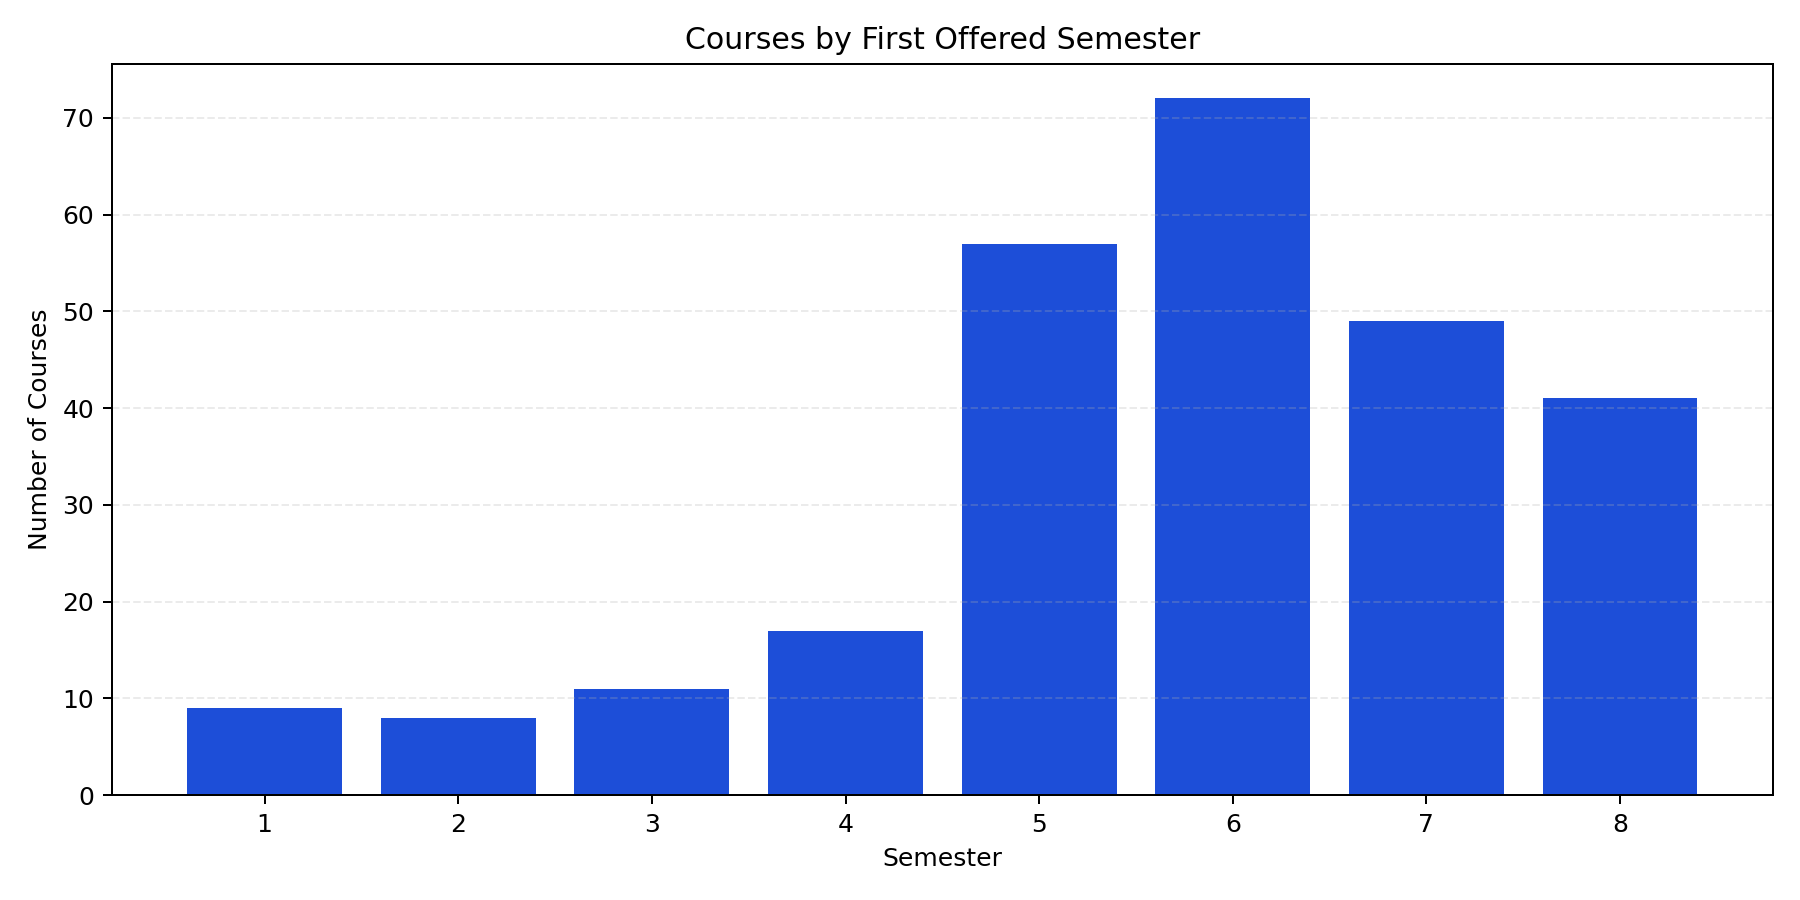
\includegraphics[width=\textwidth]{./figs/courses_by_first_semester.png}
    \end{minipage}
    \hfill
    \begin{minipage}{0.48\textwidth}
        \centering
        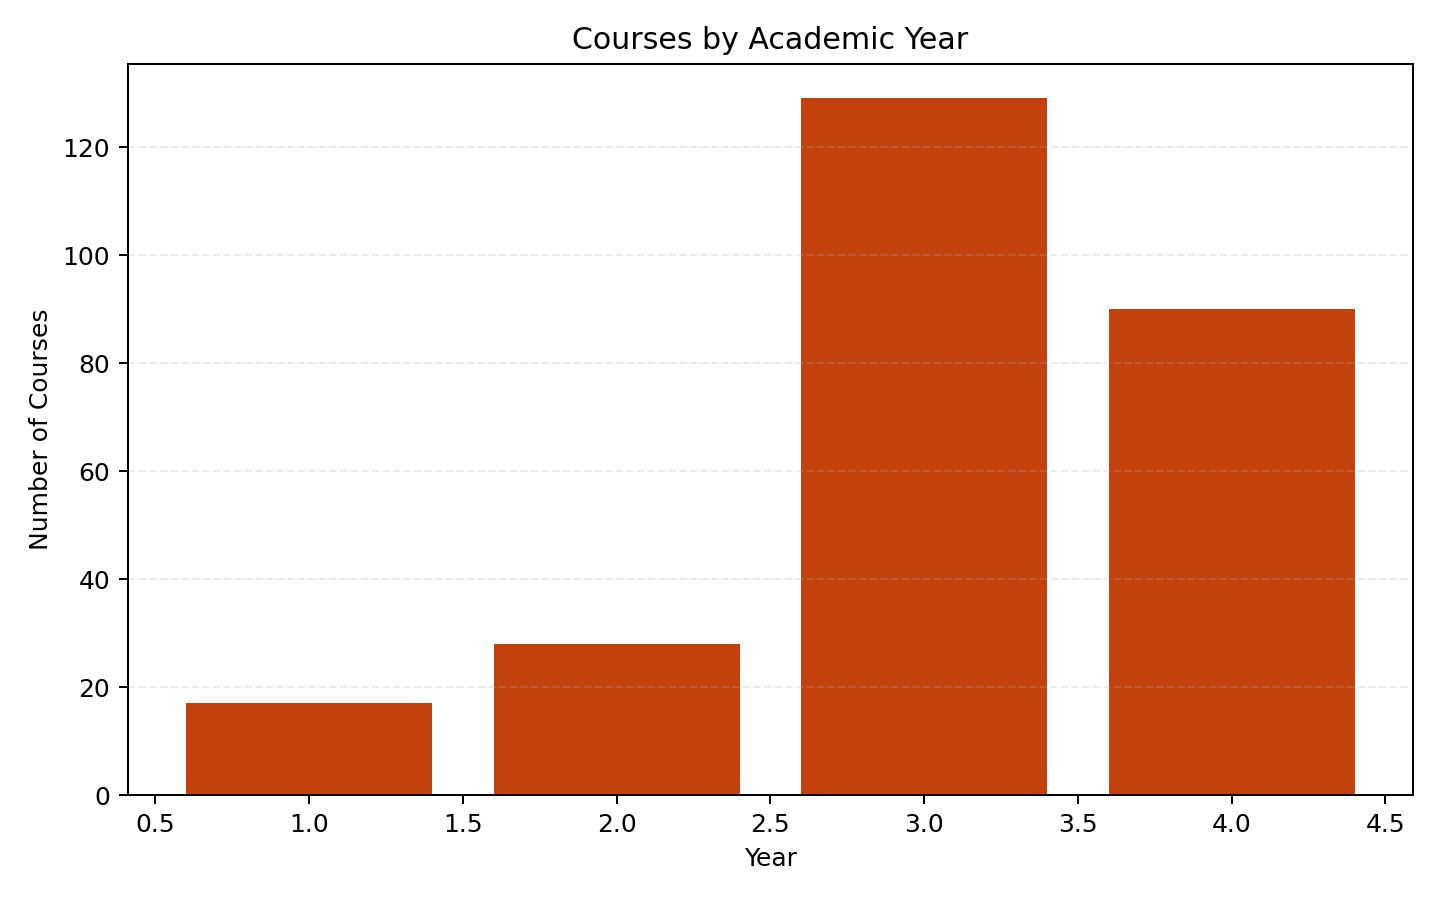
\includegraphics[width=\textwidth]{./figs/courses_by_year.png}
    \end{minipage}
    \caption{Course availability distribution over semester and academic year.}
    \label{fig:sem-year}
\end{figure}

\begin{figure}[tbp]
    \centering
    \begin{minipage}{0.48\textwidth}
        \centering
        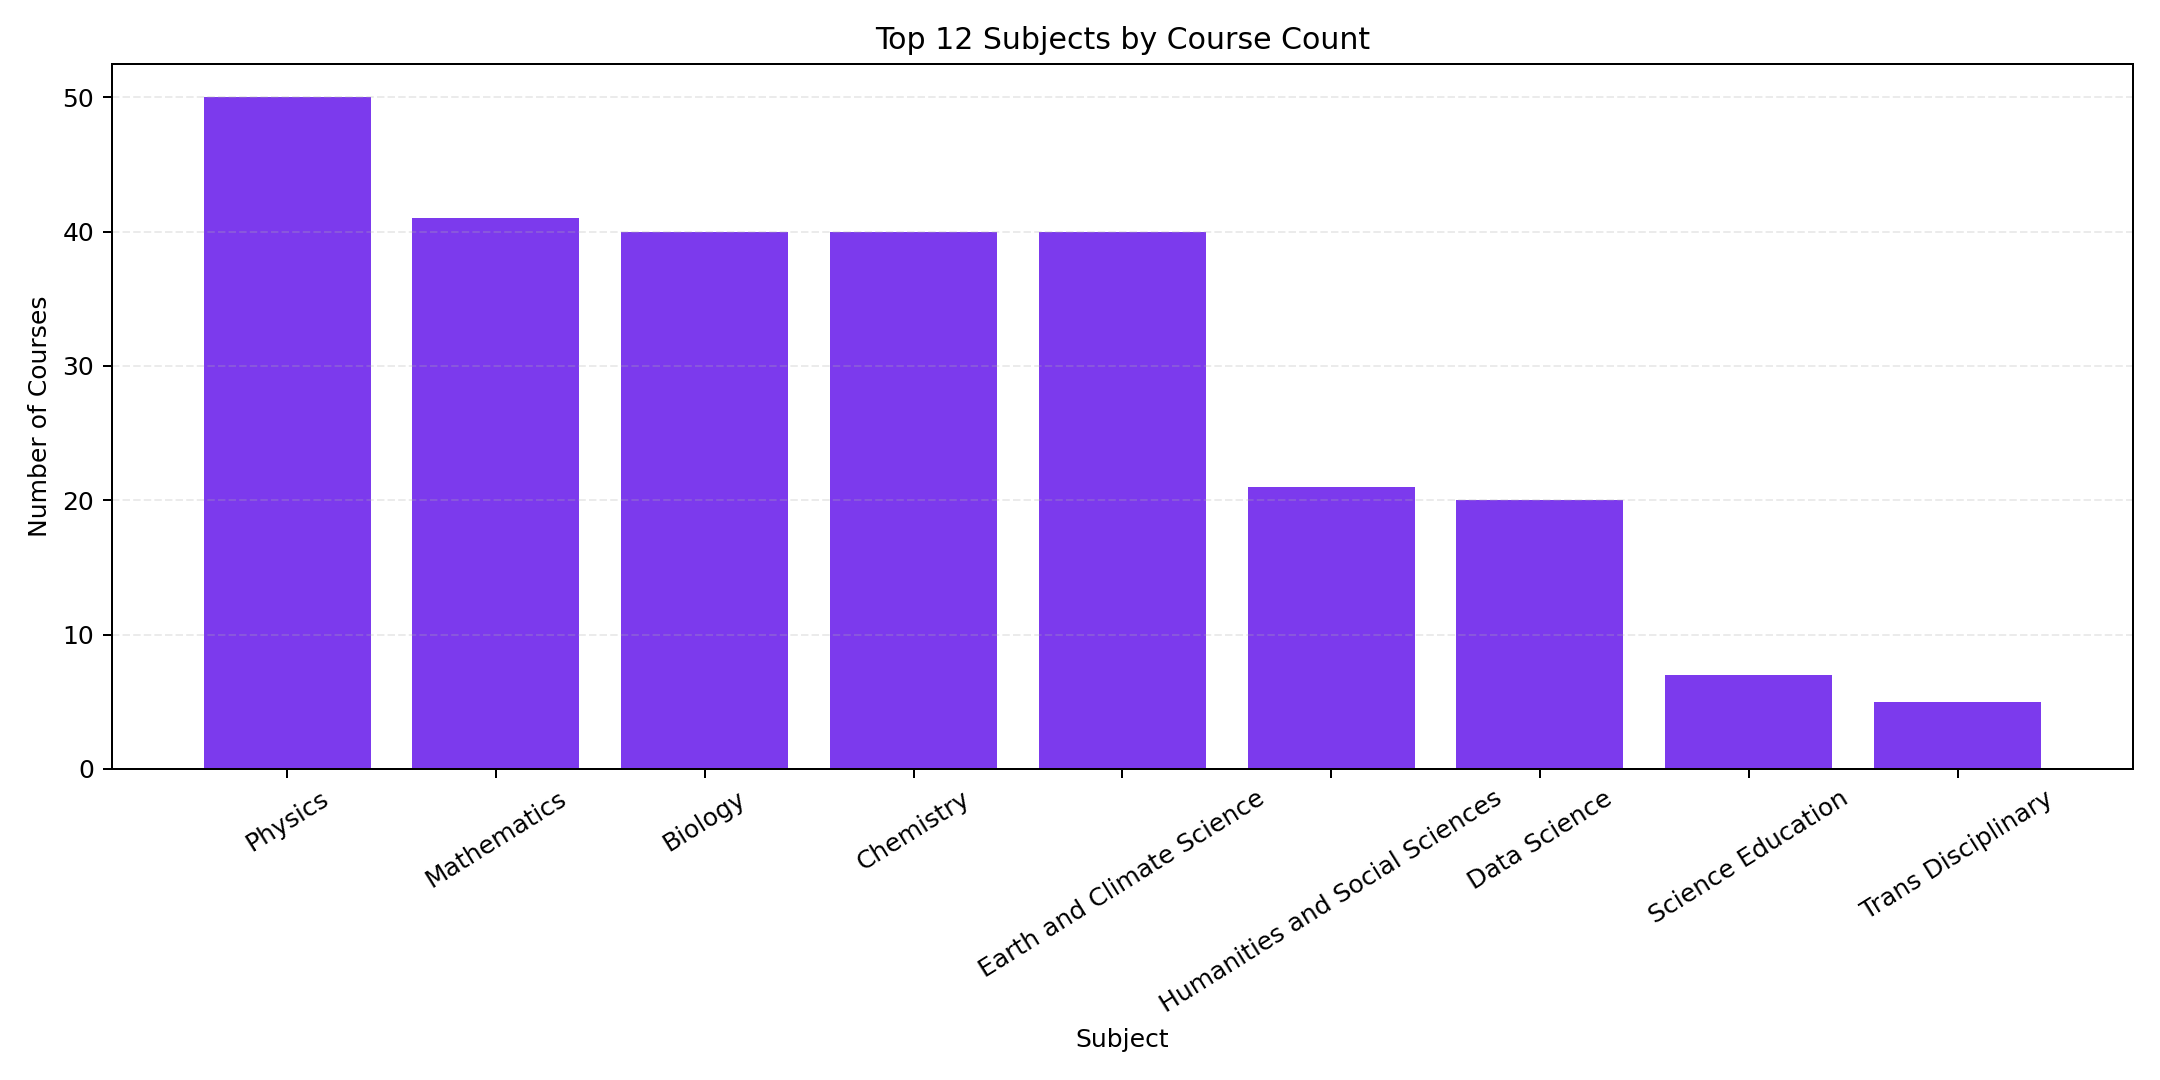
\includegraphics[width=\textwidth]{./figs/subject_distribution_top.png}
    \end{minipage}
    \hfill
    \begin{minipage}{0.48\textwidth}
        \centering
        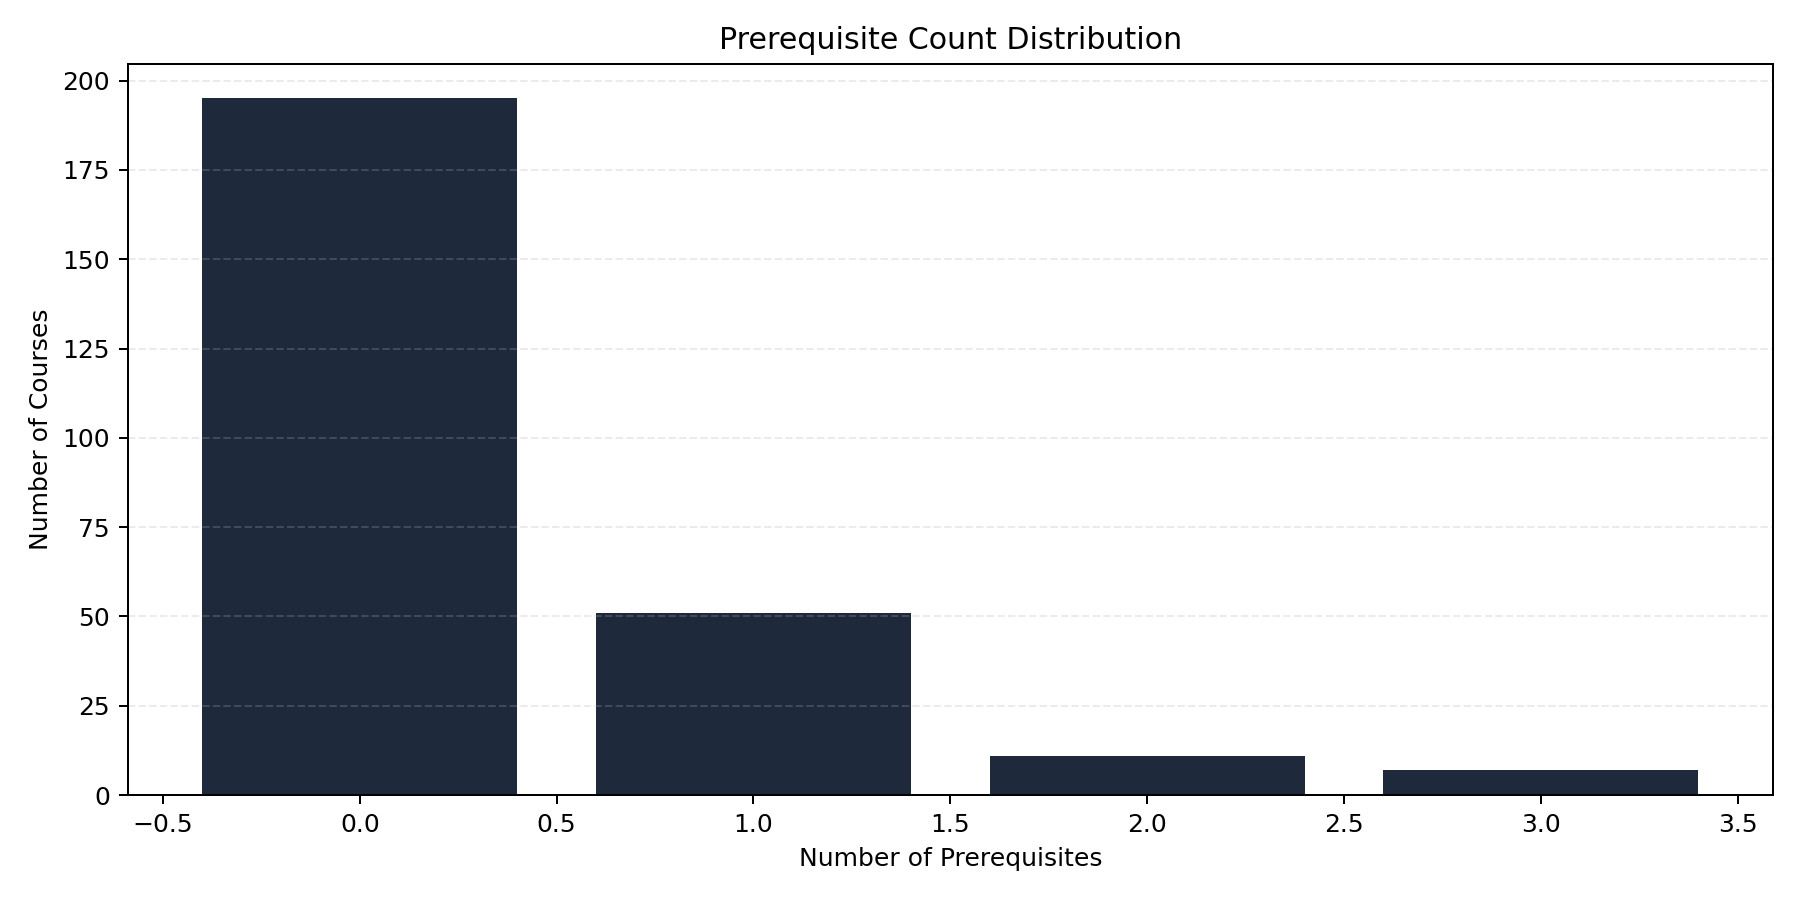
\includegraphics[width=\textwidth]{./figs/prerequisite_count_distribution.png}
    \end{minipage}
    \caption{Subject concentration and prerequisite count structure.}
    \label{fig:subject-patterns}
\end{figure}

\subsection{Dashboard Outcome}
The upgraded dashboard improves practical usability in three ways:

\begin{itemize}
    \item Cleaner student-first navigation with optional advanced tabs.
    \item Better graph readability via consistent legends, role-aware colors,
    and transition summaries.
    \item Cleaner module separation (UI vs. graph logic vs. validation) to
    support testing and maintainable iteration.
\end{itemize}

A typical student workflow is:
\begin{itemize}
    \item start in student mode and pick a major/minor program,
    \item explore the roadmap graph clustered by year and semester,
    \item inspect transition summaries to understand which semesters depend on
    earlier courses,
    \item mark completed courses and generate a constrained term plan,
    \item review blocked-course explanations when constraints prevent full
    completion.
\end{itemize}

In student testing scenarios, the planner can surface blocked courses with
unsatisfied prerequisites and propose semester-wise alternatives under credit
and load constraints.

For readability, high-resolution dashboard screenshots are included in the
Appendix as full-width figures (instead of compact side-by-side thumbnails).

\subsection{Discussion of Outcomes}
The final dashboard is not only visually cleaner but also operationally more
reliable. Key reliability and usability outcomes include:

\begin{itemize}
    \item No blocking data-quality issues in the current dataset snapshot.
    \item Stable headless startup and compile checks on the final codebase.
    \item Structured validation outputs that support testing and correctness.
    \item Better student readability through reduced clutter and clearer graph
    semantics.
\end{itemize}

\subsection{Limitations}
\begin{itemize}
    \item The semester planner is a greedy, constraint-based heuristic; it
    produces feasible schedules when possible but does not guarantee a globally
    optimal plan.
    \item Outputs depend on the accuracy and completeness of the JSON snapshot
    (course offerings, prerequisite lists, and program rules). Changes in the
    catalog or handbook rules require updating these inputs.
    \item Some prerequisite checks are policy-driven (strict/advisory/off) and
    do not model co-requisites or timetable-level constraints (e.g., clashes).
    \item Very dense graphs can still be visually complex; the dashboard
    mitigates this via filters and clarity controls, but readability may vary
    with program size.
\end{itemize}

\section{Conclusion and Outlook}
Curriculum Graph Studio now functions as a complete planning and analytics
stack: data quality checks, dependency graphs, constrained planning, pathway
validation, and a student-friendly dashboard UI. The most significant contribution is the
combination of graph-theoretic logic with a student-friendly interaction layer,
which makes technical analytics actionable for academic decision-making.

Future work includes:

\begin{itemize}
    \item personalized pathway recommendations based on student goals,
    \item what-if simulation for delayed/failed prerequisites,
    \item integration with institutional enrollment systems,
    \item longitudinal evaluation of advising outcomes.
\end{itemize}

\section{Acknowledgements}
We acknowledge the course and program-rule data sources provided for IISER Pune
curriculum modeling, and the open-source tools that enabled this work.

\section{Author Contributions}
\begin{itemize}
    \item Ayush Raj: UI development, testing, and codebase structuring.
    \item Malhar Patel: UI development, graph algorithms, and dependency analytics.
    \item Sankar Maharajan: Data preprocessing and graph validation.
    \item Applen Tahu: Data extraction and JSON schema design.
\end{itemize}

\section{Code availability}
Source code (GitHub): \url{https://github.com/Mal-Pat/curriculum-graph/tree/main}.

Key modules include \texttt{src/app.py} (dashboard UI), \texttt{src/graph.py}
(graph construction and planning), and \texttt{src/validate\_major\_minor.py}
(requirement validation).

\section{How to Run (Streamlit Dashboard)}
The dashboard is designed to be clone-safe and runnable locally with Python and
Streamlit.

\subsection{Clone and install}
\begin{enumerate}
    \item Clone the repository and enter it:
    \begin{verbatim}
git clone https://github.com/Mal-Pat/curriculum-graph.git
cd curriculum-graph
    \end{verbatim}

    \item Create and activate a virtual environment (macOS/Linux):
    \begin{verbatim}
python -m venv .venv
source .venv/bin/activate
    \end{verbatim}

    \item Install dependencies:
    \begin{verbatim}
python -m pip install --upgrade pip
python -m pip install -r requirements.txt
    \end{verbatim}
\end{enumerate}

\subsection{Run the app}
\begin{verbatim}
python -m streamlit run src/app.py
\end{verbatim}

\noindent Notes:
\begin{itemize}
    \item Default dataset path: \texttt{data/IISER-P/}.
    \item Use \textit{Student mode} for simplified navigation and graph defaults.
    \item Enable \textit{Advanced analysis tabs} for cycle checks, topological
    ordering, reachability analysis, and detailed validation/data quality.
\end{itemize}

For a quick headless smoke test:
\begin{verbatim}
python -m streamlit run src/app.py --server.headless true --server.port 8522
\end{verbatim}

% --------------------------------------------------------------------
% --------------------------------------------------------------------
% ---- DO NOT CHANGE THIS BLOCK OF CODE
\section{References}
\bibliography{refs}
% --------------------------------------------------------------------
% --------------------------------------------------------------------


\section{Appendix}

\subsection{Additional figures}
\begin{figure}[tbp]
    \centering
    \begin{minipage}{0.48\textwidth}
        \centering
        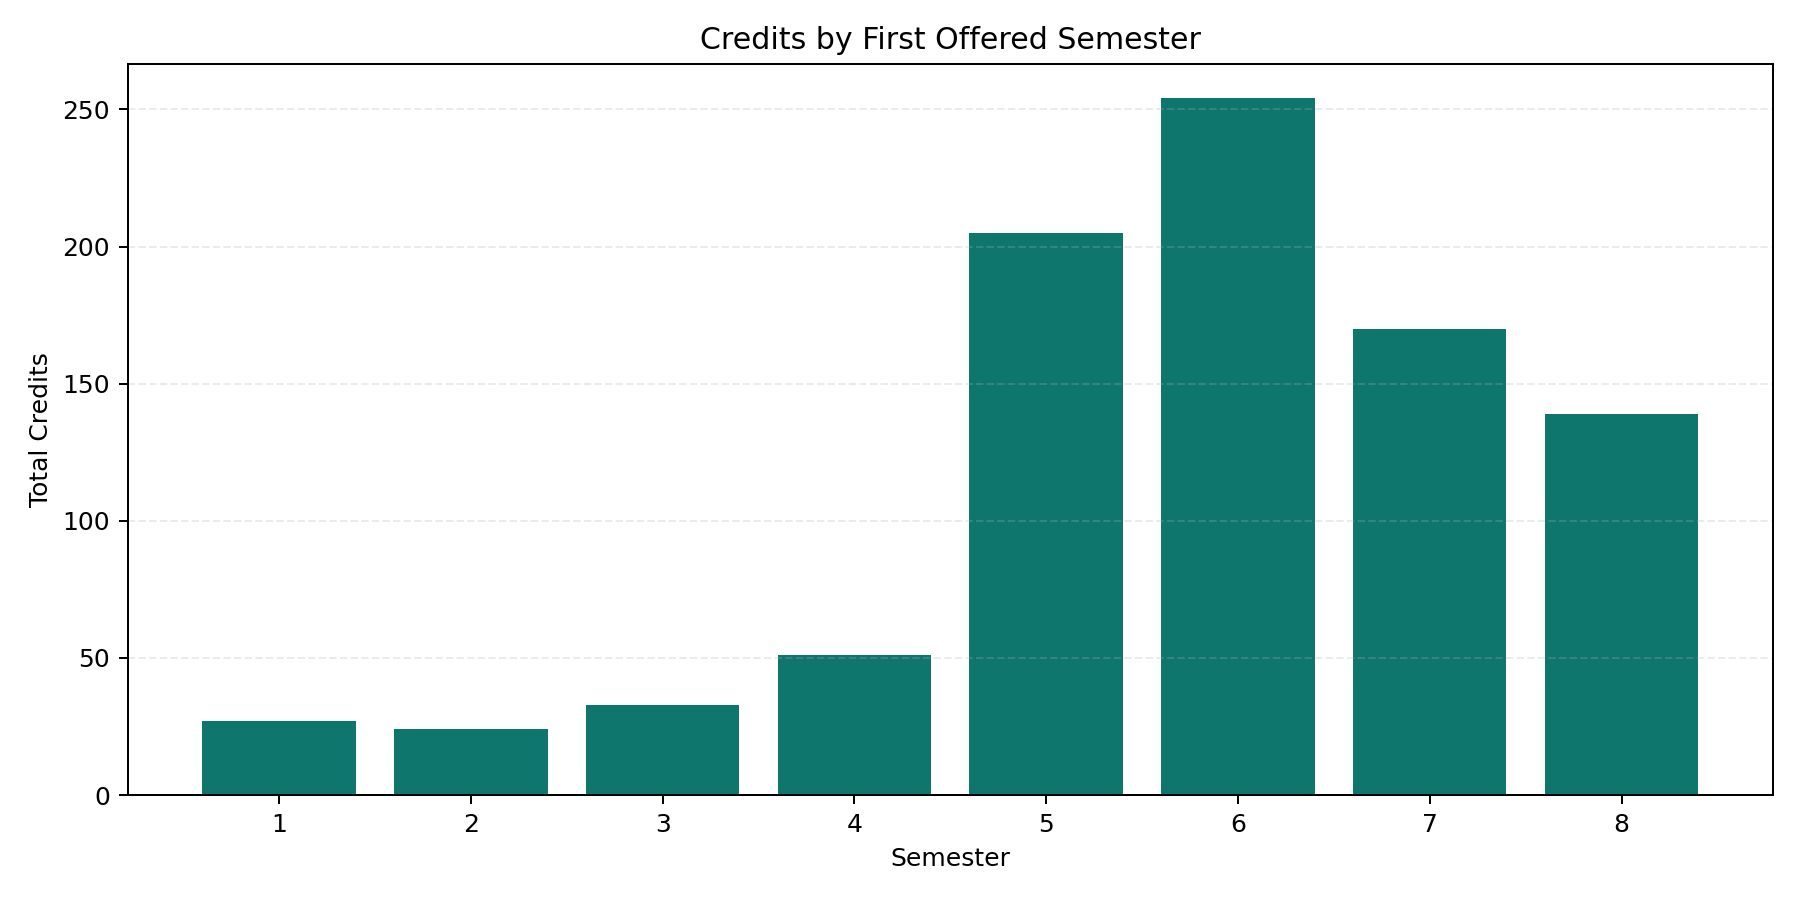
\includegraphics[width=\textwidth]{./figs/credits_by_first_semester.png}
    \end{minipage}
    \hfill
    \begin{minipage}{0.48\textwidth}
        \centering
        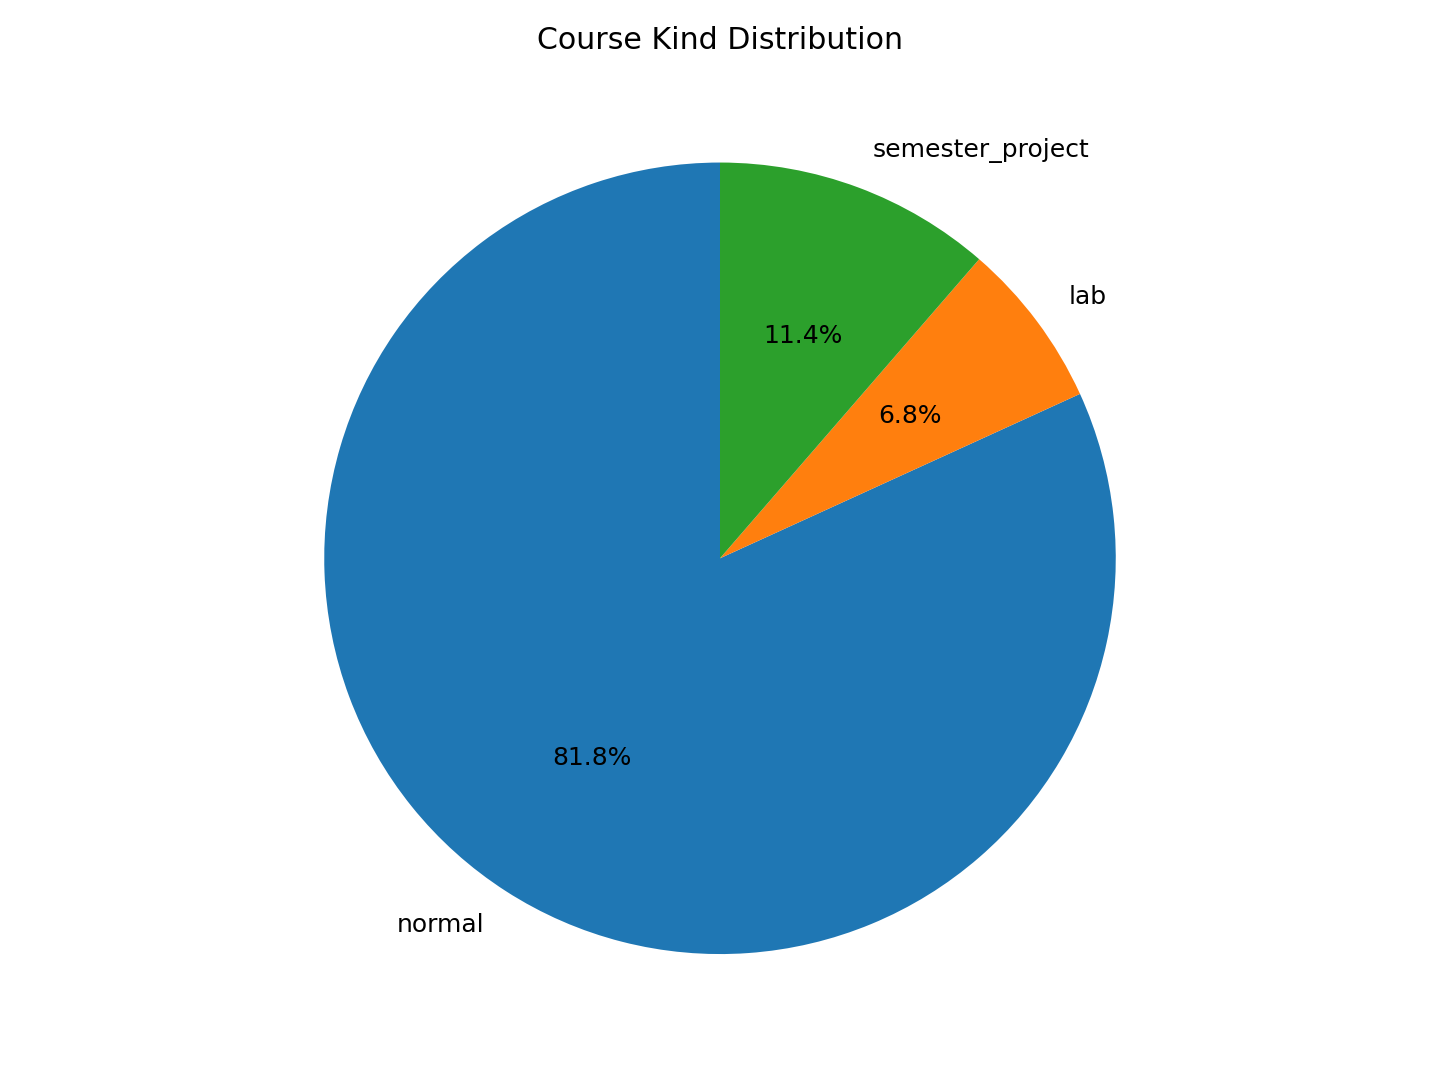
\includegraphics[width=\textwidth]{./figs/kind_distribution.png}
    \end{minipage}
    \caption{Credit load trend and course-kind distribution.}
\end{figure}


\begin{figure}[tbp]
    \centering
    \IfFileExists{./figs/graph_look_1.png}{%
        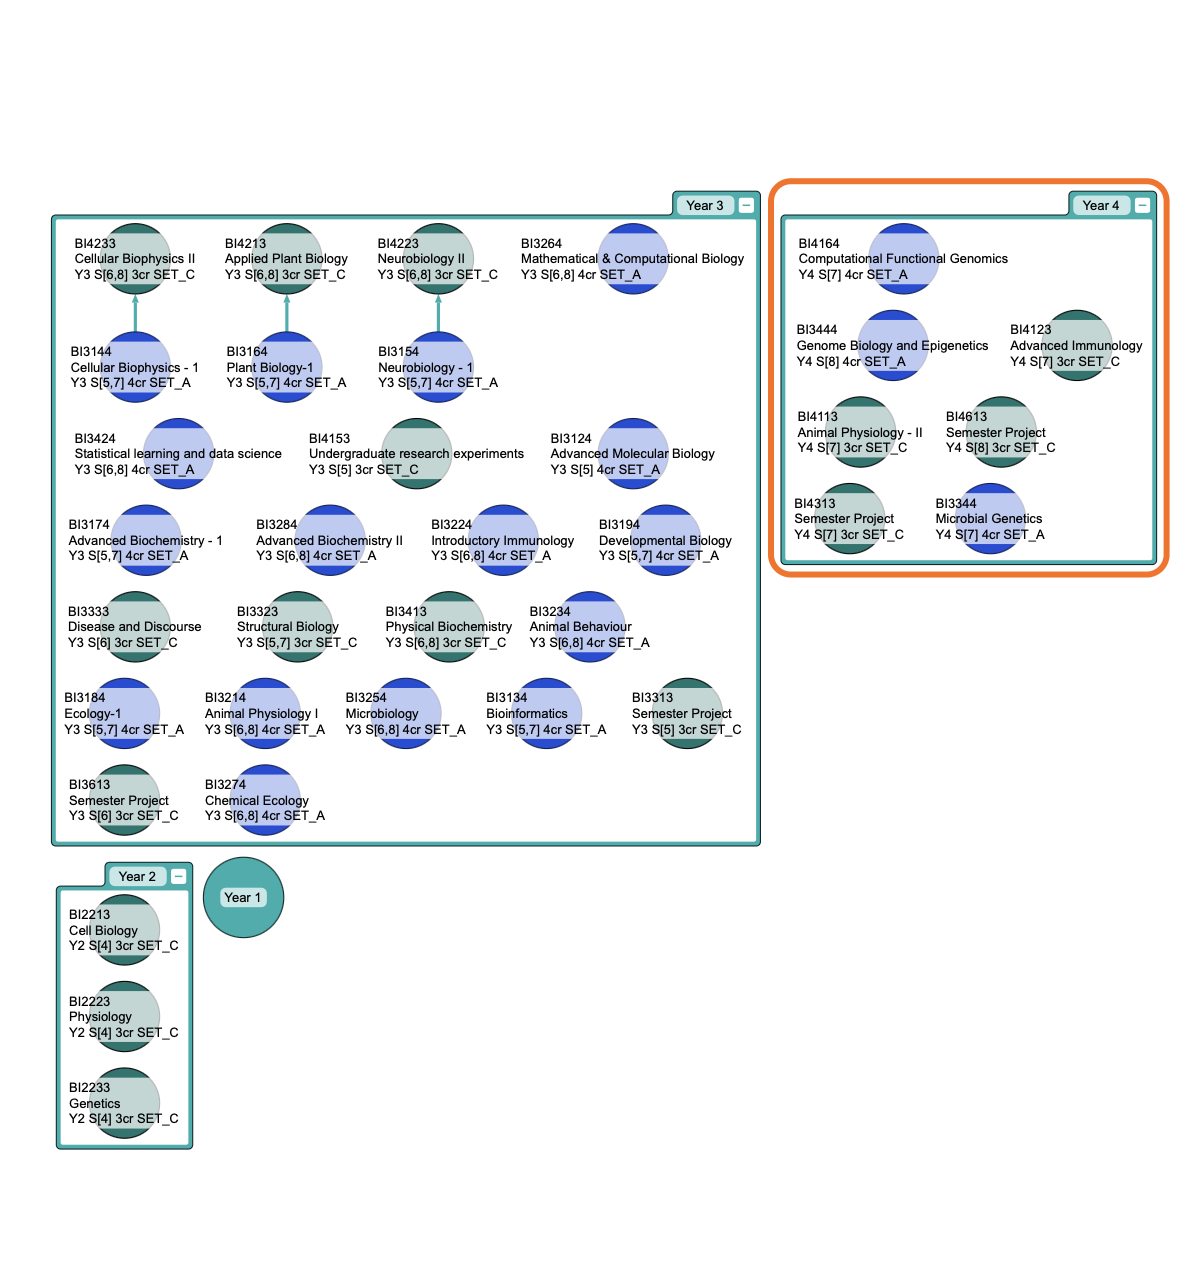
\includegraphics[width=0.95\textwidth,trim={40 110 15 160},clip]{./figs/graph_look_1.png}%
    }{%
        \fbox{\parbox[c][0.45\textwidth][c]{0.9\textwidth}{\centering
            Missing figure:\\
            \path{./figs/graph_look_1.png}
        }}%
    }
    \caption{Year-wise prerequisite graph view showing set labels and reduced clutter (dashboard screenshot).}
\end{figure}


\begin{figure}[tbp]
    \centering
    \IfFileExists{./figs/graph_look_2.png}{%
        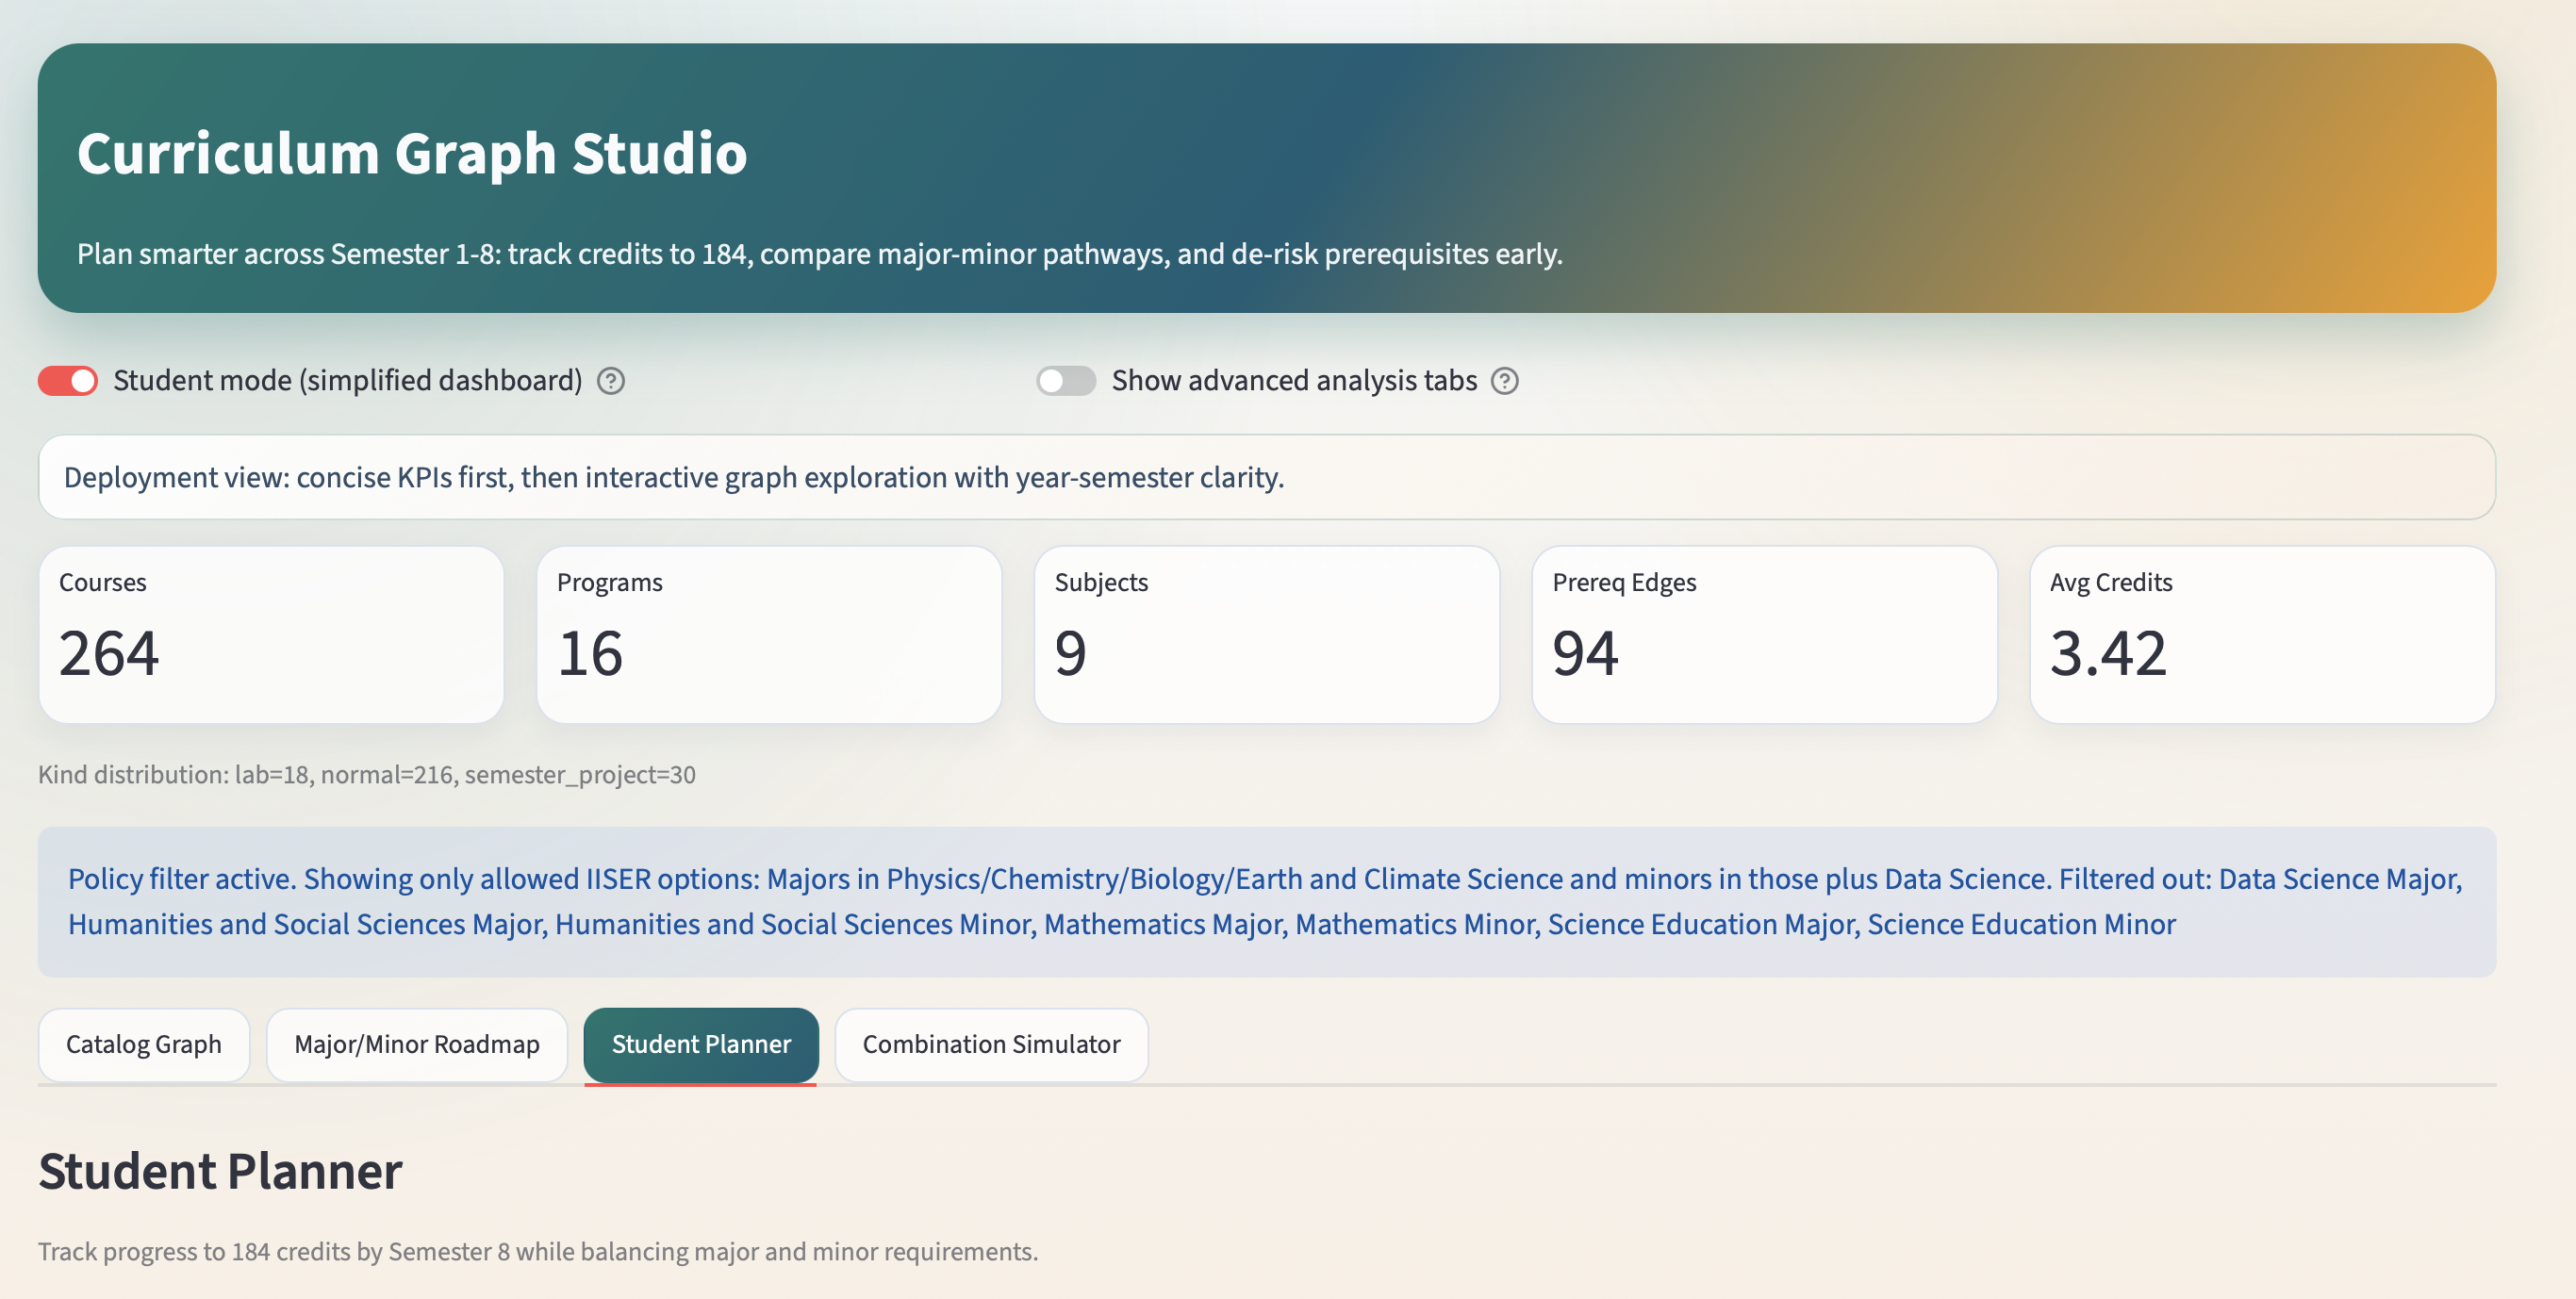
\includegraphics[width=0.95\textwidth,trim={20 30 20 20},clip]{./figs/graph_look_2.png}%
    }{%
        \IfFileExists{./figs/grapg look2.png}{%
            \includegraphics[width=0.95\textwidth,trim={20 30 20 20},clip]{./figs/grapg look2.png}%
        }{%
            \fbox{\parbox[c][0.45\textwidth][c]{0.9\textwidth}{\centering
                Missing figure:\\
                \path{./figs/graph_look_2.png}\\
                (or)\\
                \path{./figs/grapg look2.png}
            }}%
        }%
    }
    \caption{Student-mode dashboard overview showing KPIs, policy filtering, and the planner entry point.}
\end{figure}



\subsection{Algorithms}
\begin{minipage}{0.7\textwidth}
    \begin{algorithm}[H]
        \caption{Constrained Semester Planner}\label{alg:planner}
        \begin{algorithmic}
        \Require Directed graph $G$, course index $I$, start semester $s_0$, term caps
        \Ensure Semester plan $P$ and blocked set $B$
            \State Initialize completed set $C$ from known history
            \For{$s = s_0$ to planning horizon}
                \State Find feasible set $F_s = \{c \mid c \in \mathcal{O}(s) \wedge pred(c) \subseteq C\}$
                \State Rank $F_s$ by priority and downstream dependency impact
                \State Select courses under course-count and credit caps
                \State Add selected courses to $P[s]$ and update $C$
            \EndFor
            \State $B \gets V(G) \setminus C$
            \State \Return $P, B$
        \end{algorithmic}
    \end{algorithm}
\end{minipage}


% --------------------------------------------------------------------
% --------------------------------------------------------------------
% ---- DO NOT CHANGE THIS BLOCK OF CODE
\end{document}
% --------------------------------------------------------------------
% --------------------------------------------------------------------
